\documentclass[11pt]{article}

% parameters are fairly self-explanatory here, thankfully
\usepackage[width=7in,height=9.5in,top=0.75in,centering]{geometry}

% for math-ing
\usepackage{amsmath}
\usepackage{amssymb}


%%%%%% tables %%%%%%%%

\usepackage{array}
\renewcommand{\arraystretch}{1.5}
\setlength{\tabcolsep}{8pt}

%%%%%% plotting %%%%%%

\usepackage[dvipsnames]{xcolor}
\usepackage{tikz}
\usepackage{pgfplots}

\pgfplotsset{every axis/.append style={
                    axis x line=middle,    % put the x axis in the middle
                    axis y line=middle,    % put the y axis in the middle
                    axis line style={<->,color=black}, % arrows on the axis
                    xlabel={$x$},          % default put x on x-axis
                    ylabel={$y$},          % default put y on y-axis
            }}
            
 \pgfplotsset{compat=1.14} % sometimes, everything falls apart without this
 
 %\usepgfplotslibrary{fillbetween} %for shading between curves

%%%%%% commands %%%%%%

% exam heading; course name is first argument, exam information is second argument
\newcommand{\Heading}[2]{
    \fbox{
        {\Large\textbf{#1}}
        }
    \hfill
    \fbox{
        \begin{minipage}{0.2\textwidth}
            \begin{center}
            \textbf{#2}
            \end{center}
        \end{minipage}
    }
    \par\vspace{0.1in}}

% for being lazy while beautifying integrals
\newcommand{\dint}{\displaystyle\int}

% for being lazy while beautifying limits
\newcommand{\dlim}{\displaystyle\lim}

%%%%%% stuff %%%%%%

\usepackage{fancyhdr}

\setcounter{page}{0} % first page is page 0

\parindent0pt % no indent

\fboxsep=0.25cm % little space in fbox border

%%%%%% BEGIN! %%%%%%%

\begin{document}

\pagestyle{fancy}

% record goals here to create sense of transparency

\fancyhead[c]{%
  \ifcase\value{page}
  % empty test for page = 0
  \or
  \or {\bf\color{ProcessBlue} F1: Lines \& Slope}% page=1
  \or {\bf\color{RoyalBlue} L1: Limits and Continuity}% page = 2
  \or {\bf\color{RoyalBlue} L2: Evaluating Limits Using Continuity and Forms}% page = 3
  \or {\bf\color{ForestGreen} D1: Meaning of a Derivative}% page = 4
  \or
  \else
  % Empty chead here!
  \fi
}

\thispagestyle{empty} % don't display that this is page 0

\Heading{MATH 1190/1210 Survey of Calculus I}{Knowledge Checkpoint 1\\Solutions\\Fall 2025}

\vspace{0.1in}

\textbf{Name} \hrulefill \, \textbf{Date} \hrulefill\\

\begin{minipage}{0.16\textwidth}\begin{center}\textbf{UVA ID\\ (e.g. hdj4nd)} \end{center}\end{minipage}\hrulefill \, \begin{minipage}{0.2\textwidth}\begin{center}\textbf{Course \&\\ Section Number} \end{center}\end{minipage} \hrulefill\\

\hrulefill
\paragraph*{Course \& Section Numbers:}

{\small
\begin{center}
\begin{tabular}{| c | c | c | c | c |}
\hline
%
\begin{minipage}{0.12\textwidth}\begin{center}
1190-100\\
J. Rolf\\
(12:30 PM)
\end{center}\end{minipage}
&
\begin{minipage}{0.12\textwidth}\begin{center}
1190-200\\
J. Rolf\\
(2 PM)
\end{center}\end{minipage}
&
\begin{minipage}{0.12\textwidth}\begin{center}
1210-100\\
Mikhail\\
(8 AM)
\end{center}\end{minipage}
&
\begin{minipage}{0.12\textwidth}\begin{center}
1210-200\\
Raul\\
(9:30 AM)
\end{center}\end{minipage}
&
\begin{minipage}{0.12\textwidth}\begin{center}
1210-300\\
David\\
(11 AM)
\end{center}\end{minipage}
\\
%
\hline
%
\begin{minipage}{0.12\textwidth}\begin{center}
1210-400\\
David\\
(12:30 PM)
\end{center}\end{minipage}
&
\begin{minipage}{0.12\textwidth}\begin{center}
1210-500\\
Michael\\
(2 PM)
\end{center}\end{minipage}
&
\begin{minipage}{0.12\textwidth}\begin{center}
1210-600\\
J. Rolf\\
(3:30 PM)
\end{center}\end{minipage}
&
\begin{minipage}{0.12\textwidth}\begin{center}
1210-700\\
Josh\\
(9:30 AM)
\end{center}\end{minipage}
&
\begin{minipage}{0.12\textwidth}\begin{center}
1210-800\\
Mason\\
(2 PM)
\end{center}\end{minipage}
\\
%
\hline
%
\begin{minipage}{0.12\textwidth}\begin{center}
1210-900\\
Caelan\\
(3:30 PM)
\end{center}\end{minipage}
&
\begin{minipage}{0.12\textwidth}\begin{center}
1210-920\\
Caelan\\
(5 PM)
\end{center}\end{minipage}
&
\begin{minipage}{0.12\textwidth}\begin{center}
1210-940\\
Mitchell\\
(10 AM)
\end{center}\end{minipage}
&
\begin{minipage}{0.12\textwidth}\begin{center}
1210-950\\
Mitchell\\
(11 AM)
\end{center}\end{minipage}
&
\begin{minipage}{0.12\textwidth}\begin{center}
1210-960\\
Mitchell\\
(noon)
\end{center}\end{minipage}
\\
\hline
\end{tabular}
\end{center}

}

{%\small

\paragraph*{Instructions:}

\begin{itemize}
    
    \item The regular time allowed for completing this assessment is \fbox{$40$} minutes.
    %\item This assessment is out of 50 points.\\
    \item This assessment contains prompts on the following targets: {\bf\color{ProcessBlue}F1}, {\bf\color{RoyalBlue}L1}, {\bf\color{RoyalBlue}L2}, {\bf\color{ForestGreen}D1}.
    \item On each assessment prompt, you will receive a score of Exceeds Expectations (5), Proficient (4), Almost (3), Developing (2), Emerging (1), or Not Yet (0). {\bf Please do not interpret your score as a percentage.}
    %\item You will have opportunities to reassess on the targets appearing on this assessment after the next {\bf 2} assessments.\\
    \item You may NOT use calculators, dictionaries, notes, phones, or any other kinds of aids.
    \item Please write neatly. What cannot be read, cannot be graded.
    \item Carefully work out each problem and clearly indicate your final answer to every problem.
    \item Please provide the most specific answer possible. For instance, if a limit does not exist because it goes to $\infty$ or $-\infty$, then specify this.
    \item Please use the methods discussed up to this point in the course. For example, any work based on l'H\^opital's Rule will not receive credit on this assessment.
    \item \textbf{All work must be shown unless otherwise specified.} Partial credit will not be given if appropriate work is not shown.
    \item In particular, {\bf any answer appearing with no justification will receive no credit regardless of whether the answer was correct}, unless otherwise specified.
    \item Please first respond to the items on which you feel most proficient, then respond to others later.
    \item Check your assessment before you start. There should be 5 pages containing 5 numbered items.
    \end{itemize}
    
    }

\vfill


%%%%%%%%%
\newpage\,\newpage%
%%%%%%%%%


\begin{enumerate}

%%%%%%%%%%%%%%%%%%%%%%%%%%%%%%%%%%%%%%%%%%%%%%%%%%%%%
%%%%%%%%%%% BEGIN PROBLEM F1 %%%%%%%%%%%%%%%%%%%%%%%%
%%%%%%%%%%%%%%%%%%%%%%%%%%%%%%%%%%%%%%%%%%%%%%%%%%%%%

\item Below is a table showing the relationship between the year and the total value of US imports in that year (in billion dollars).

\begin{table}[h!]
        \centering
        \begin{tabular}{|c|c|c|c|c|c|}
            \hline
            Year & 2000 & 2005 & 2010 & 2015 & 2020 \\
            \hline
            Value (in billion dollars) & 1450 & 1700 & 1960 & 2150 & 2300\\
            \hline
        \end{tabular}
    \end{table}


\begin{enumerate}
    \item What is the net change of the total value of US imports from 2005 to 2020? Make sure to include units in your final result.

    \textcolor{blue}{\textbf{Solution:} The net change is 
    \[
    2300 - 1700 = 600 \text{ billion dollars}.
    \]}

    \vfill

    \item What is the average rate of the total value of US imports from 2005 to 2020? Make sure to include units in your final result.

    \textcolor{blue}{\textbf{Solution:} The average rate is
    \[
    \frac{2300 - 1700}{2020 - 2005} = \frac{600}{15} = 40 \text{ billion dollars per year}.
    \]}

    \vfill

    \item Use a sentence or two to explain the meaning of the average rate of change \textbf{in the context of this scenario}. 
    
    Do NOT use average rate of change or slope in your explanation.

    \textcolor{blue}{\textbf{Solution:} The total value of US imports increased by 40 billion dollars on average, for each year between 2005 and 2020.}

    \vfill
\end{enumerate}

%%%%%%%%%%%%%%%%%%%%%%%%%%%%%%%%%%%%%%%%%%%%%%%%%%%%%
%%%%%%%%%%% END PROBLEM F1 %%%%%%%%%%%%%%%%%%%%%%%%%%
%%%%%%%%%%%%%%%%%%%%%%%%%%%%%%%%%%%%%%%%%%%%%%%%%%%%%

\newpage

%%%%%%%%%%%%%%%%%%%%%%%%%%%%%%%%%%%%%%%%%%%%%%%%%%%%%
%%%%%%%%%%% BEGIN PROBLEM L1 %%%%%%%%%%%%%%%%%%%%%%%%
%%%%%%%%%%%%%%%%%%%%%%%%%%%%%%%%%%%%%%%%%%%%%%%%%%%%%

\item The graph of the function is given below.
       
\begin{center}
    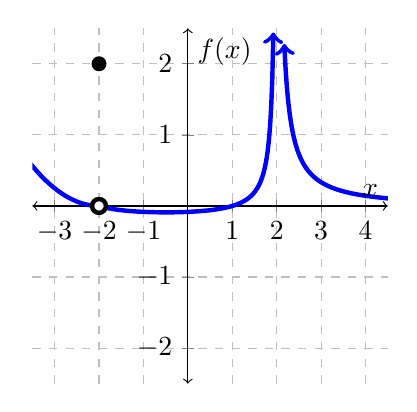
\begin{tikzpicture}[scale=1]
    \begin{axis}[
        %    axis y line = left,
        %    axis x line = bottom,
            xlabel={$x$},
            xtick       = {-3,-2,-1,1,2,3,4},
            xticklabels = {$-3$,$-2$,$-1$,$1$,$2$,$3$,$4$},
            ylabel={$f(x)$},
            ytick       = {-2,-1,1,2,3},
            yticklabels = {$-2$,$-1$,$1$,$2$,$3$},
            samples     = 160,
            domain      = -3.5:4.5,
            restrict y to domain=-2.5:2.5,
            xmin = -3.5, xmax = 4.5,
            ymin = -2.5, ymax = 2.5,
            grid=both, grid style=dashed,
            width=2.4in, height=2.4in
          ]
          \addplot[ultra thick,blue,<-, domain=-4:-2] {(1/4)*(x+2)^2};
          \addplot[ultra thick,blue,->, domain=-2:2] {-1/(x^2+x-6)-0.25};
          \addplot[ultra thick,blue,<-, domain=2:5] {2/(x^2+x-6)};
          \filldraw[fill=white,ultra thick] (-2,0) circle (2.5pt);
          \filldraw (-2,2) circle (2.5pt);
          %\node at (-2,2.5) {\fbox{C}};
    \end{axis}
    \end{tikzpicture} 
\end{center}

{\bf You must explain your answers to receive credit. Write all correct answer choices.} \hfill\,

\begin{enumerate}

\item On the interval $[-3, 4]$, at what $a$-value(s) does the limit $\lim\limits_{x\to a}f(x)$ NOT exist? For each value you write down, explain why the limit doesn't exist.

\textcolor{blue}{\textbf{Solution:} On the interval $[-3,4]$, $\displaystyle \lim_{x\to a}f(x)$ does not exist at $x = 2$. As x approaches 2 from either side, f(x) grows without bound, so cannot approach any real number.}
\vspace{2in}

\item On the interval $[-3, 4]$, at what $a$-value(s) is $f(x)$ NOT continuous at $x=a$? For each point where there is a discontinuity, determine its type and explain why it belongs to that type.
\textcolor{blue}{\textbf{Solution:} On the interval $[-3,4]$, $f(x)$ is not continuous at $x = -2$, which is a removable discontinuity. So the function value is not equal to the limit (i.e. even though the function is defined at $x = -2$ and $ \displaystyle \lim_{x \to -2} f(x)$ exists, $\displaystyle \lim_{x \to-2} f(x) \neq f(-2)$). It is also the case that $f(x)$ is not continuous at $x = 2$, which is an infinite discontinuity. Here, $f(2)$ is not defined, $\displaystyle \lim_{x \to 2}f(x)$ does not exist  (again, it increases without bound from either side so cannot be a finite number) and $\displaystyle \lim_{x \to2} f(x) \neq f(2)$).}
 

\end{enumerate}

%%%%%%%%%%%%%%%%%%%%%%%%%%%%%%%%%%%%%%%%%%%%%%%%%%%%%
%%%%%%%%%%% END PROBLEM L1 %%%%%%%%%%%%%%%%%%%%%%%%%%
%%%%%%%%%%%%%%%%%%%%%%%%%%%%%%%%%%%%%%%%%%%%%%%%%%%%%

\newpage

%%%%%%%%%%%%%%%%%%%%%%%%%%%%%%%%%%%%%%%%%%%%%%%%%%%%%
%%%%%%%%%%% BEGIN PROBLEM L2 %%%%%%%%%%%%%%%%%%%%%%%%
%%%%%%%%%%%%%%%%%%%%%%%%%%%%%%%%%%%%%%%%%%%%%%%%%%%%%

\item Evaluate the following limits using continuity or form.

If you use continuity to evaluate a limit, to receive full credit, please provide sufficient explanation for why continuity can be used, including why the given function is continuous at the given point.

If you use form to evaluate a limit, to receive full credit, please list the form and show all steps. 

% DJ's wording: For each limit below, first find the form of the limit, then find the value of the limit. If the given function is continuous at the target, then you may simply write ``n/a" for the form. Show complete work - using mathematics and/or words - to accompany your answers.
\begin{enumerate}
    \item \(\displaystyle \lim_{x\to -2}\frac{3x+5}{\sqrt{x+4}}\)

    \vspace{4pt}

    \textcolor{blue}{\textbf{Solution:} \\
    \textbf{Form:} n/a (the function is continuous at \(x=-2\)).\\[4pt]
    The numerator \(3x+5\) is a polynomial, its domain is all real numbers so it is defined everywhere (in particular at $x = -2$). For the denominator since $x = -2$ is in its domain, \(\sqrt{x+4}\) is also defined at \(x=-2\). Additionally, the denominator is not zero when $x = -2$. Hence, by the Main Continuity Theorem, the quotient is continuous at \(x=-2\). By the definition of continuity we may evaluate the limit by direct substitution:
    \[
      \lim_{x\to -2}\frac{3x+5}{\sqrt{x+4}}=\frac{3(-2)+5}{\sqrt{-2+4}}=\frac{-1}{\sqrt{2}}
      =-\frac{\sqrt{2}}{2}.
    \]
    }


    \item \(\displaystyle \lim_{x\to -2^{+}}\frac{3x+5}{\sqrt{x+2}}\)

    \vspace{4pt}

    \textcolor{blue}{\textbf{Solution:} \\ 
    \textbf{Form:} \(\dfrac{c}{0}\) .\\[4pt]
    Evaluate the numerator and check the behavior of the denominator as \(x\to -2^{+}\):
    \[
      3x+5 \to 3(-2)+5=-1,
      \qquad \sqrt{x+2}\to 0.
    \]
    Note \(\sqrt{x+2}\) is defined only for \(x\ge -2\); for \(x>-2\) we have \(\sqrt{x+2}>0\). Thus as \(x\to -2^+\),
    \[
      \frac{3x+5}{\sqrt{x+2}}\; \to \;\frac{-1}{\text{small}^+}\;\longrightarrow\;-\infty.
    \]
    So the right-hand limit is \(\displaystyle\lim_{x\to -2^+}\frac{3x+5}{\sqrt{x+2}}=-\infty\). 
    }
\end{enumerate}


%%%%%%%%%%%%%%%%%%%%%%%%%%%%%%%%%%%%%%%%%%%%%%%%%%%%%
%%%%%%%%%%% END PROBLEM L2 %%%%%%%%%%%%%%%%%%%%%%%%%%
%%%%%%%%%%%%%%%%%%%%%%%%%%%%%%%%%%%%%%%%%%%%%%%%%%%%%

\newpage

%%%%%%%%%%%%%%%%%%%%%%%%%%%%%%%%%%%%%%%%%%%%%%%%%%%%%
%%%%%%%%%%% BEGIN PROBLEM D1 %%%%%%%%%%%%%%%%%%%%%%%%
%%%%%%%%%%%%%%%%%%%%%%%%%%%%%%%%%%%%%%%%%%%%%%%%%%%%%

\item The figure below shows the power output, $p(w)$, of a wind turbine as a function of wind speed $w$. The units of $w$ and $p$ are also shown in the figure.

\begin{center}
    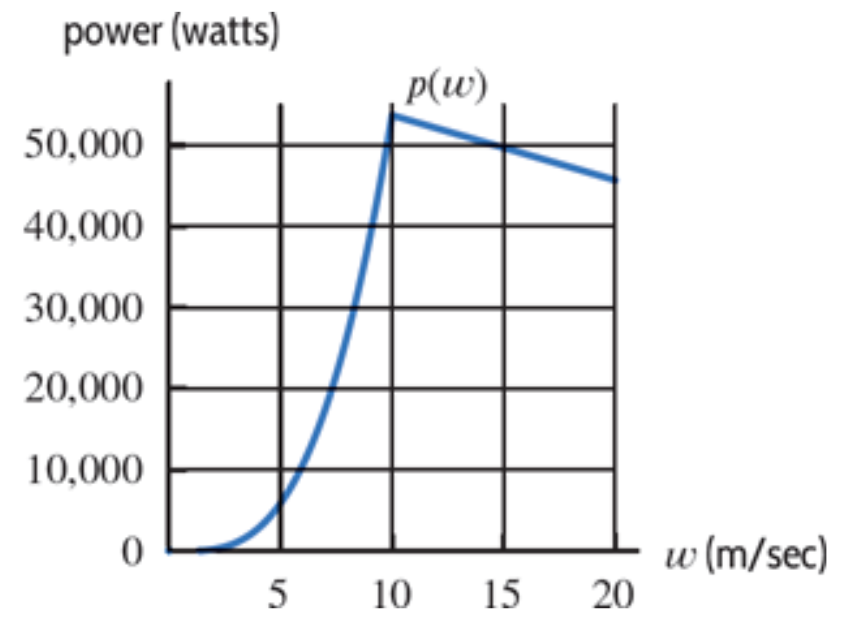
\includegraphics[scale=0.5]{KC1D1}
\end{center}
\begin{enumerate}
    \item Use a sentence or two to explain the meaning of the equation $p(15)=50000$ in this context. 
    To receive full credit, please include units for all quantities discussed, and do not include any mathematical terms such as ``limit" or ``instantaneous rate of change".
    \vspace{6pt}

    \textcolor{blue}{\textbf{Solution:} At a wind speed of 15 meters per second, the wind turbine produces 50,000 watts of power. This means that when the wind blows at 15 m/s, the power output of the turbine is 50,000 W.}

    \vfill 

    \item Use a sentence or two to explain the meaning of the equation $p'(15)=-8000$ in this context. 
    To receive full credit, please include units for all quantities discussed, and do not include any mathematical terms such as ``limit" or ``instantaneous rate of change".
    \vspace{4pt}

    \textcolor{blue}{\textbf{Solution:} At a wind speed of 15 meters per second, the power output of the wind turbine is decreasing at a rate of 8,000 watts per meter per second. This means that if the power output were to change exactly as it did when the wind speed was 15 m/sec for every 1 m/s increase in wind speed beyond 15 m/s, the turbine’s power output would drop by 8,000 W.}

    \vfill

    \item What is $p'(10)$? To receive full credit, explain why.

    \vspace{4pt}

    \textcolor{blue}{\textbf{Solution:} $p'(10)=DNE$. The limiting behavior of the slopes of secant lines between the points $w = 10$ and a point $w_0 \neq 10$ do not agree as $w_0 \to 10$ from either side of the graph (i.e. $\displaystyle \lim_{w \to 10^{+}} \frac{p(w) - p(10)}{w - 10} \neq \lim_{w \to 10^{-}} \frac{p(w) - p(10)}{w - 10}$). Approaching from the left-hand side the slopes are approaching an increasingly larger positive number while approaching from the right-hand side, the slopes are always negative. So, this limit does not exist when $w = 10$, which means the derivative does not exist when $w = 10$}.
    
\end{enumerate}



%%%%%%%%%%%%%%%%%%%%%%%%%%%%%%%%%%%%%%%%%%%%%%%%%%%%%
%%%%%%%%%%% END PROBLEM D1 %%%%%%%%%%%%%%%%%%%%%%%%%%
%%%%%%%%%%%%%%%%%%%%%%%%%%%%%%%%%%%%%%%%%%%%%%%%%%%%%

\newpage

This page is left blank intentionally.\\

Use this page if you need additional space to write your solutions to any problem. \\

If you wish this page graded, you must refer to this page on \textbf{the original page} of the problem. Otherwise, your grader will NOT consider your work on this page.

\end{enumerate}

\end{document}